\documentclass{article}



\usepackage[utf8]{inputenc}
\usepackage{longtable}
\usepackage{authblk}
\usepackage{adjustbox}

\usepackage{natbib}

% autores
\title{LOS INDICES DE COLOMBIA}


\renewcommand\Authand{, y }
\author[1]{\normalsize ANDRES MARIN}

\affil[1]{\small  Escuela de Ingeniería,Universidad de los Andes\\
\texttt{{ja.marin11}@uniandes.edu.co}}

\date{29 de Junio de 2018}





\usepackage{Sweave}
\begin{document}
\Sconcordance{concordance:ProyectoFINAL.tex:ProyectoFINAL.Rnw:%
1 27 1 1 0 18 1 1 7 7 1 1 5 15 0 1 2 8 1 1 8 1 4 7 1 1 7 1 3 8 1 1 6 12 %
0 1 2 4 1 1 8 13 0 1 2 6 1 1 3 1 2 2 1 1 5 3 1 1 4 31 0 1 2 10 1 1 13 1 %
1 1 39 3 1 1 29 1 2 9 1}


\maketitle


\begin{abstract}
Este es mi primer trabajo en exploracion y modelamiento de indices usando LATEX. Este trabajo lo he hecho bajo la filosofía de trabajo replicable. Este es mi primer trabajo en exploracion y modelamiento de indices usando LATEX. Este trabajo lo he hecho bajo la filosofía de trabajo replicable. Este es mi primer trabajo en exploracion y modelamiento de indices usando LATEX. Este trabajo lo he hecho bajo la filosofía de trabajo replicable. Este es mi primer trabajo en exploracion y modelamiento de indices usando LATEX. Este trabajo lo he hecho bajo la filosofía de trabajo replicable.
\end{abstract}

\section*{Introducción}

Aqui les presento mi investigacion sobre diversos indices sociales en el mundo. Los indices los conseguí de wikipedia, espero que les gusten mucho. Aqui les presento mi investigacion sobre diversos indices sociales en el mundo. Los indices los conseguí de wikipedia, espero que les gusten mucho.Aqui les presento mi investigacion sobre diversos indices sociales en el mundo. Los indices los conseguí de wikipedia, espero que les gusten mucho.Aqui les presento mi investigacion sobre diversos indices sociales en el mundo. Los indices los conseguí de wikipedia, espero que les gusten mucho.
Aqui les presento mi investigacion sobre diversos indices sociales en el mundo. Los indices los conseguí de wikipedia, espero que les gusten mucho.Aqui les presento mi investigacion sobre diversos indices sociales en el mundo. Los indices los conseguí de wikipedia, espero que les gusten mucho.Aqui les presento mi investigacion sobre diversos indices sociales en el mundo. Los indices los conseguí de wikipedia, espero que les gusten mucho.

Comencemos viendo que hay en la sección \ref{univariada} en la página \pageref{univariada}.

\clearpage


\section{Exploración Univariada}\label{univariada}


\begin{abstract}
Este es mi primer trabajo en exploracion y modelamiento de indices usando LATEX. Este trabajo lo he hecho bajo la filosofía de trabajo replicable. Este es mi primer trabajo en exploracion y modelamiento de indices usando LATEX. Este trabajo lo he hecho bajo la filosofía de trabajo replicable. Este es mi primer trabajo en exploracion y modelamiento de indices usando LATEX. Este trabajo lo he hecho bajo la filosofía de trabajo replicable. Este es mi primer trabajo en exploracion y modelamiento de indices usando LATEX. Este trabajo lo he hecho bajo la filosofía de trabajo replicable.
\end{abstract}

% Table created by stargazer v.5.2.2 by Marek Hlavac, Harvard University. E-mail: hlavac at fas.harvard.edu
% Date and time: Fri, Jun 29, 2018 - 23:47:49
\begin{table}[!htbp] \centering 
  \caption{Medidas estadísticas} 
  \label{stats} 
\begin{tabular}{@{\extracolsep{5pt}}lcc} 
\\[-1.8ex]\hline 
\hline \\[-1.8ex] 
Statistic & \multicolumn{1}{c}{N} & \multicolumn{1}{c}{Median} \\ 
\hline \\[-1.8ex] 
IDH & 32 & 0.804 \\ 
Poblacion.Cabecera & 32 & 717,197 \\ 
Poblacion.Resto & 32 & 268,111.5 \\ 
Poblacion.Total & 32 & 1,028,429 \\ 
\hline \\[-1.8ex] 
\end{tabular} 
\end{table} 


\begin{abstract}
Este es mi primer trabajo en exploracion y modelamiento de indices usando LATEX. Este trabajo lo he hecho bajo la filosofía de trabajo replicable. Este es mi primer trabajo en exploracion y modelamiento de indices usando LATEX. Este trabajo lo he hecho bajo la filosofía de trabajo replicable. Este es mi primer trabajo en exploracion y modelamiento de indices usando LATEX. Este trabajo lo he hecho bajo la filosofía de trabajo replicable. Este es mi primer trabajo en exploracion y modelamiento de indices usando LATEX. Este trabajo lo he hecho bajo la filosofía de trabajo replicable.
\end{abstract}


\centering
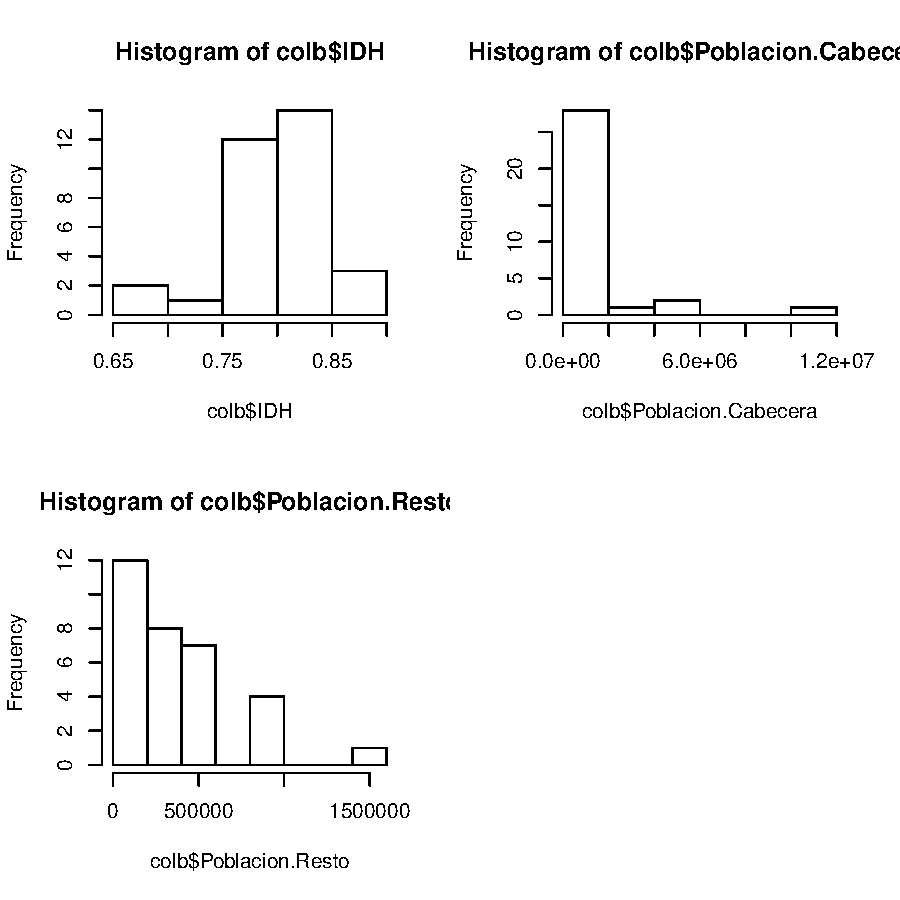
\includegraphics{ProyectoFINAL-barplots}



\begin{abstract}
Este es mi primer trabajo en exploracion y modelamiento de indices usando LATEX. Este trabajo lo he hecho bajo la filosofía de trabajo replicable. Este es mi primer trabajo en exploracion y modelamiento de indices usando LATEX. Este trabajo lo he hecho bajo la filosofía de trabajo replicable. Este es mi primer trabajo en exploracion y modelamiento de indices usando LATEX. Este trabajo lo he hecho bajo la filosofía de trabajo replicable. Este es mi primer trabajo en exploracion y modelamiento de indices usando LATEX. Este trabajo lo he hecho bajo la filosofía de trabajo replicable.
\end{abstract}

\centering
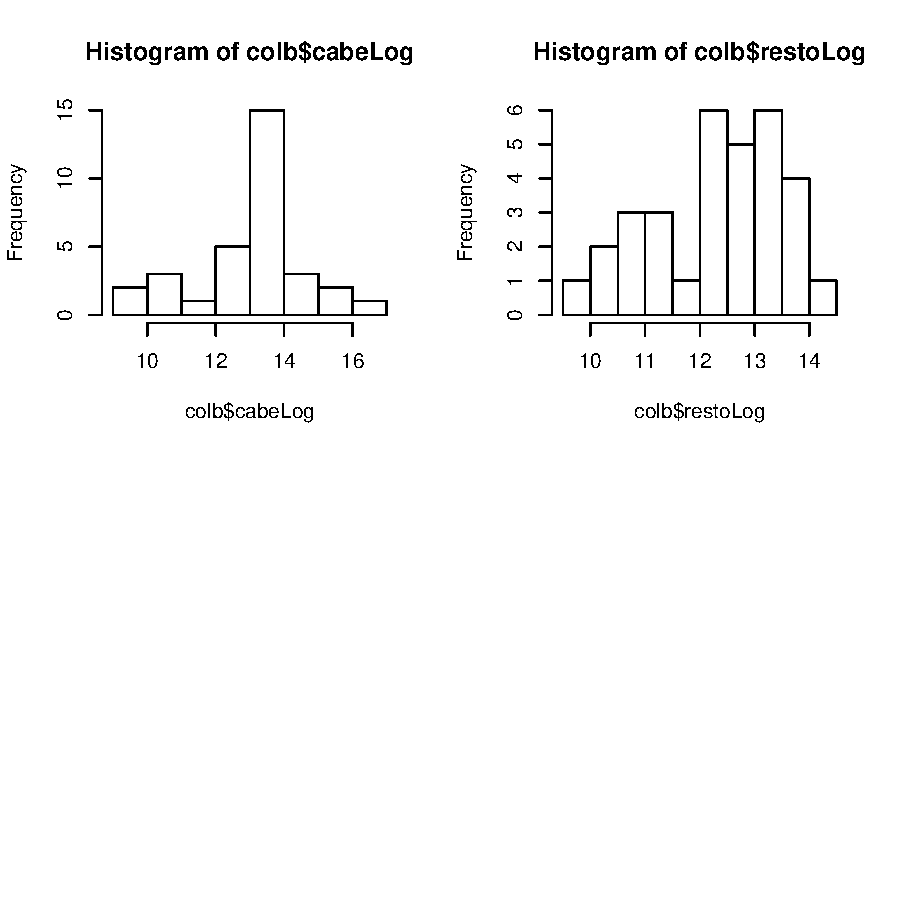
\includegraphics{ProyectoFINAL-barplots2}
\section{Exploración Bivariada}\label{bivariada}
\clearpage


\begin{abstract}
Este es mi primer trabajo en exploracion y modelamiento de indices usando LATEX. Este trabajo lo he hecho bajo la filosofía de trabajo replicable. Este es mi primer trabajo en exploracion y modelamiento de indices usando LATEX. Este trabajo lo he hecho bajo la filosofía de trabajo replicable. Este es mi primer trabajo en exploracion y modelamiento de indices usando LATEX. Este trabajo lo he hecho bajo la filosofía de trabajo replicable. Este es mi primer trabajo en exploracion y modelamiento de indices usando LATEX. Este trabajo lo he hecho bajo la filosofía de trabajo replicable.
\end{abstract}

\centering
% Table created by stargazer v.5.2.2 by Marek Hlavac, Harvard University. E-mail: hlavac at fas.harvard.edu
% Date and time: Fri, Jun 29, 2018 - 23:47:52
\begin{table}[!htbp] \centering 
  \caption{Correlación de Democracia con las demás variables} 
  \label{corrDem} 
\begin{tabular}{@{\extracolsep{5pt}} cc} 
\\[-1.8ex]\hline 
\hline \\[-1.8ex] 
cabeLog & restoLog \\ 
\hline \\[-1.8ex] 
$0.560$ & $0.269$ \\ 
\hline \\[-1.8ex] 
\end{tabular} 
\end{table} 
\begin{abstract}
Este es mi primer trabajo en exploracion y modelamiento de indices usando LATEX. Este trabajo lo he hecho bajo la filoso
\end{abstract}
\centering
% Table created by stargazer v.5.2.2 by Marek Hlavac, Harvard University. E-mail: hlavac at fas.harvard.edu
% Date and time: Fri, Jun 29, 2018 - 23:47:52
\begin{table}[!htbp] \centering 
  \caption{correlación entre las variables independientes} 
  \label{corrDem1} 
\begin{tabular}{@{\extracolsep{5pt}} ccc} 
\\[-1.8ex]\hline 
\hline \\[-1.8ex] 
 & cabeLog & restoLog \\ 
\hline \\[-1.8ex] 
cabeLog & $1$ & $0.840$ \\ 
restoLog & $0.840$ & $1$ \\ 
\hline \\[-1.8ex] 
\end{tabular} 
\end{table} 

\begin{abstract}
Este es mi primer trabajo en exploracion y modelamiento de indices usando LATEX. Este trabajo lo he hecho bajo la filosofía de trabajo replicable. Este es mi primer trabajo en exploracion y modelamiento de indices usando LATEX. Este trabajo lo he hecho bajo la filosofía de trabajo replicable. Este es mi primer trabajo en exploracion y modelamiento 

\end{abstract}
\centering
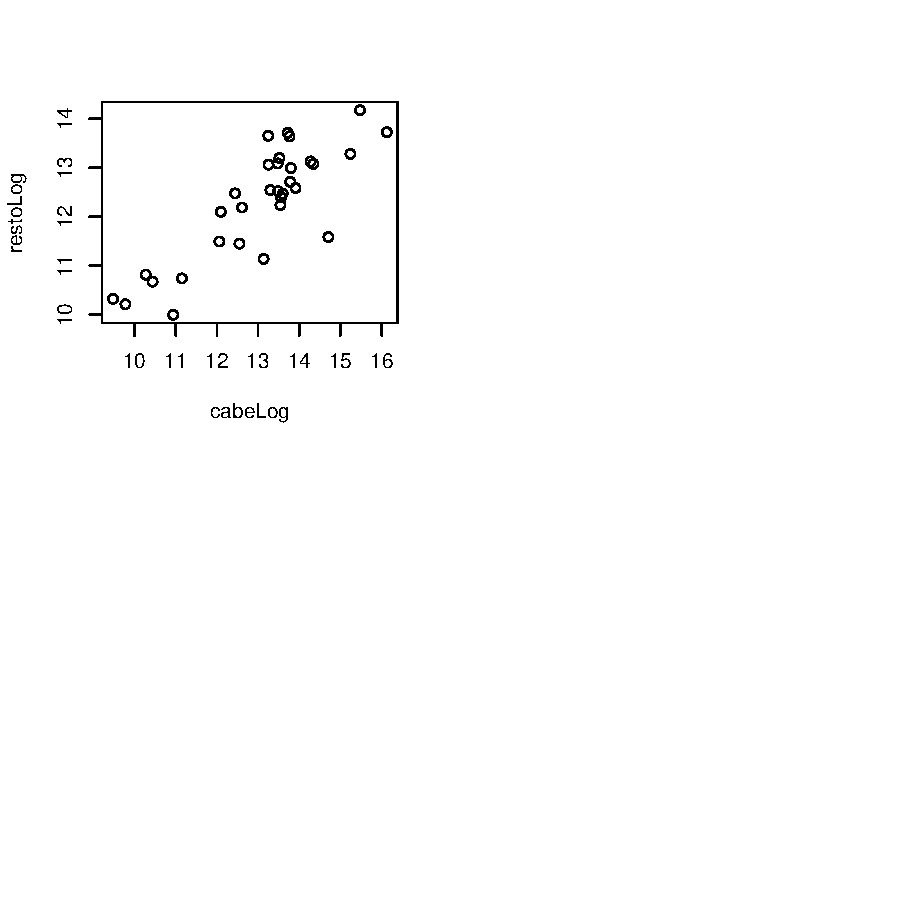
\includegraphics{ProyectoFINAL-barplots4}


\centering



\centering
% Table created by stargazer v.5.2.2 by Marek Hlavac, Harvard University. E-mail: hlavac at fas.harvard.edu
% Date and time: Fri, Jun 29, 2018 - 23:47:52
\begin{table}[!htbp] \centering 
  \caption{Modelos de Regresión} 
  \label{regresiones} 
\begin{tabular}{@{\extracolsep{5pt}}lcc} 
\\[-1.8ex]\hline 
\hline \\[-1.8ex] 
 & \multicolumn{2}{c}{\textit{Dependent variable:}} \\ 
\cline{2-3} 
\\[-1.8ex] & \multicolumn{2}{c}{IDH} \\ 
\\[-1.8ex] & (1) & (2)\\ 
\hline \\[-1.8ex] 
 cabeLog & 0.016$^{***}$ & 0.034$^{***}$ \\ 
  & (0.004) & (0.007) \\ 
  & & \\ 
 restoLog &  & $-$0.029$^{**}$ \\ 
  &  & (0.010) \\ 
  & & \\ 
 Constant & 0.584$^{***}$ & 0.712$^{***}$ \\ 
  & (0.058) & (0.070) \\ 
  & & \\ 
\hline \\[-1.8ex] 
Observations & 32 & 32 \\ 
R$^{2}$ & 0.314 & 0.455 \\ 
Adjusted R$^{2}$ & 0.291 & 0.417 \\ 
Residual Std. Error & 0.040 (df = 30) & 0.036 (df = 29) \\ 
F Statistic & 13.701$^{***}$ (df = 1; 30) & 12.103$^{***}$ (df = 2; 29) \\ 
\hline 
\hline \\[-1.8ex] 
\textit{Note:}  & \multicolumn{2}{r}{$^{*}$p$<$0.1; $^{**}$p$<$0.05; $^{***}$p$<$0.01} \\ 
\end{tabular} 
\end{table} 


\section{Exploración Espacial}\label{espacial}

\begin{abstract}
Este es mi primer trabajo en exploracion y modelamiento de indices usando LATEX. Este trabajo lo he hecho bajo la filosofía de trabajo replicable. Este es mi primer trabajo en exploracion y modelamiento de indices usando LATEX. Este trabajo lo he hecho bajo la filosofía de trabajo replicable. Este es mi primer trabajo en exploracion y modelamiento de indices usando LATEX. Este trabajo lo he hecho bajo la filosofía de trabajo replicable. Este es mi primer trabajo en exploracion y modelamiento de indices usando LATEX. Este trabajo lo he hecho bajo la filosofía de trabajo replicable.
\end{abstract}






\begin{figure}[h]
\centering
\begin{adjustbox}{width=6cm,height=4cm,clip,trim=1cm 2.5cm 0cm 2.5cm}
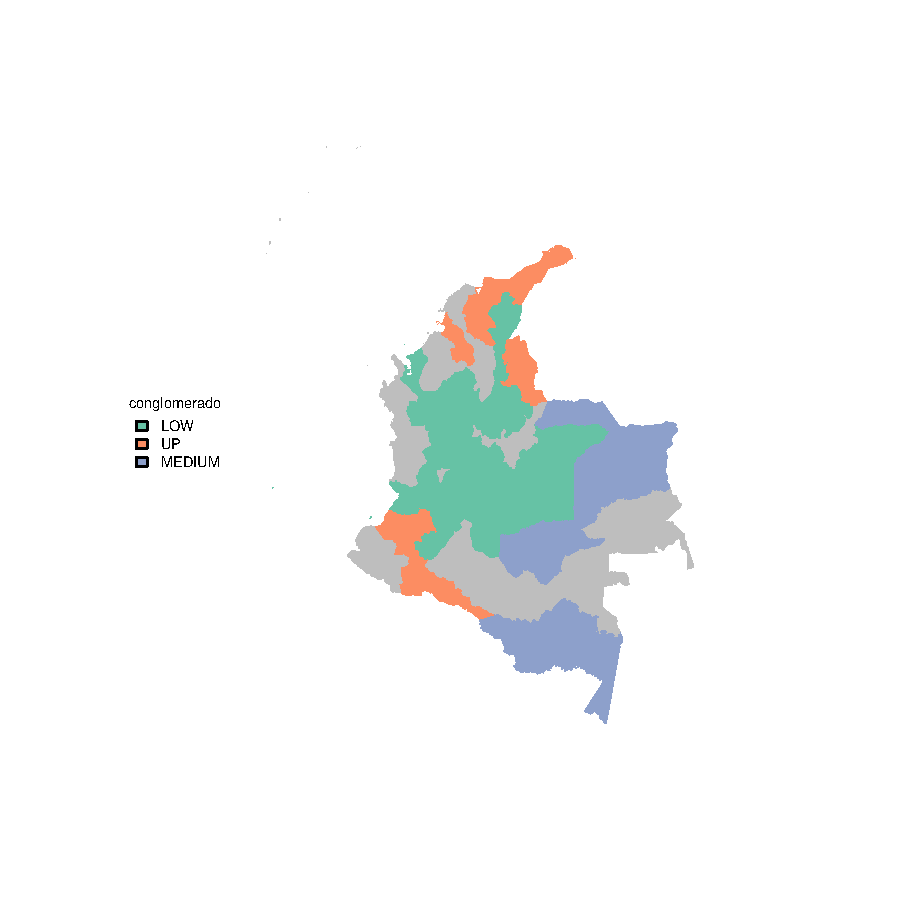
\includegraphics{ProyectoFINAL-getMapconglomerado}
\end{adjustbox}
\caption{Paises conglomerados segun sus indicadores sociopolíticos}\label{clustmap}
\end{figure}


% \bibliographystyle{abbrv}
% \renewcommand{\refname}{Bibliografia}
% % #\bibliography{MACQUEEN}

\end{document}
